\documentclass[10pt,b5paper,papersize,dvipdfmx]{jsbook}

\usepackage{vuccaken}
\usepackage{vuccaken2019}

% スタイルファイルの読み込みや自作マクロは、
% 最終的には vuccaken2019.sty の中に書いてください。
% とりあえずはここに書いてもらって構いません。


\begin{document} % 以下本文

% - - - - - - - - - - - - - - - - - - - - - - - - %
\kaishititle%
  {磁気単極子を考慮した電磁気学}% title
  {物理科学科一回生}% 所属
  {福田大和}% name
% - - - - - - - - - - - - - - - - - - - - - - - - %

% \setcounter{tocdepth}{2} % 目次にどこまで表示するか
% \tableofcontents % 目次出力
% \clearpage % 改ページ

%
\section*{はじめに}


\section{具体例}
では、実際に具体例をいくつか考えていきます。
\subsection{例1}
磁気単極子が単独である状況を考えます。これは至極単純で、磁場を$\mathbf{B}$、磁荷を$q_m$とすると、磁気単極子から距離$r$の点Pでの磁場は、
\begin{align}
\mathbf{B_P}(\mathbf{r})=\frac{q_m}{4\pi\mu}\frac{\mathbf{r}}{|\mathbf{r}|^3}
\end{align}
これを任意の閉曲面$S$(ただし、閉曲面の内側に磁気単極子を含む)で積分してやれば、
\begin{align}
\label{eq:Gaussjm}
\mathbf{B}(\mathbf{r})=\frac{q_m}{\mu}
\end{align}
となり、磁場についてのマクスウェル方程式と矛盾が生じてしまいます。よって、磁気単極子を仮定するならば、磁場についてのガウスの法則を\shiki{Gaussjm}で置き換えてやればよいように思われます。
\subsection{例2}
磁気単極子と電子が距離$a$だけ離れて存在するときを考えます。

\section{一般論}
ここからは、一般論をお話ししていきたいと思います。

% \begin{figure}[htbp]
%   \centering
%   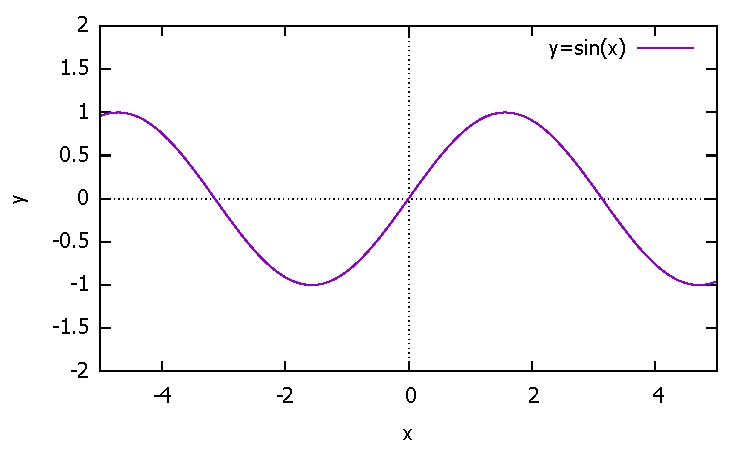
\includegraphics[width=10cm]{temp/fig-sin.pdf}
%   \caption{$y=\sin x$のグラフ。gnuplotで作成した。}
%   \label{fig:sin}
% \end{figure}

%% 参考文献
\begin{thebibliography}{9}
\bibitem{mechanics} 戸田 盛和,『物理入門コース 力学』,岩波書店,2017/12/5
\bibitem{Maxwel} 小宮山 進・竹川 敦,『マクスウェル方程式から始める電磁気学』,裳華房,2016/9/15 第二版

\end{thebibliography}

\end{document}
